\problemname{Färgrobot}

En robot kan röra sig längs en rad av färgade rutor. Varje ruta kan
vara antingen röd, grön eller blå. Ett kommando till roboten utgörs av
en färg. Roboten rör sig då åt höger och stannar när den hamnar på
färgen som kommandot angav. Skriv ett program som, för en given följd
av rutor och ett tal $N$ skriver ut den sekvens av $N$ kommandon som
gör att roboten tar sig så långt till höger som möjligt.

\begin{figure}[ht!]
\centering
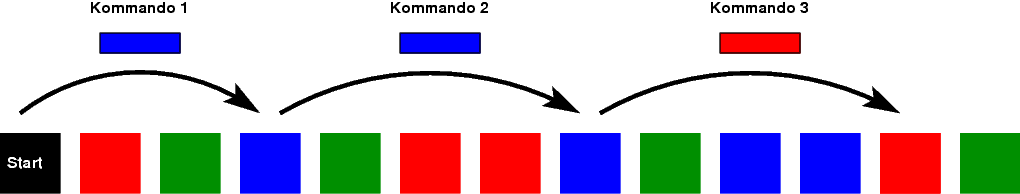
\includegraphics[width=0.8\textwidth]{fargrobot.png}
\caption{En illustration av det tredje exemplet.}
\label{overflow}
\end{figure}


\section*{Input}
Den första raden innehåller ett heltal $N$, antalet kommandon du ska
ge roboten. Den andra raden innehåller en sträng av bokstäver, R, G eller B, som
anger färgen på varje ruta i raden, från vänster till höger. Strängen är mindre än
200 tecken lång, och alltid tillräckligt lång för att ingen sekvens
av $N$ kommandon kan få roboten att nå utanför raden av rutor.

\section*{Output}

Programmet ska skriva ut en sträng med $N$ bokstäver, vardera R, G
eller B, som utgör sekvensen av kommandon du ska ge roboten för att
den ska komma så långt som möjligt i raden med rutor. Om det finns
flera sekvenser som åstadkommer detta kan du ange vilken som helst av dem.

\section*{Gränser}

\begin{enumerate}
\item I ett testfall värt 20 poäng är $N=4$ och sekvensen är
  'RGBGGBGRBRBRGRGRB' (d.v.s. fallet som angavs på årets PO-affisch)
\item I ytterligare testfall värda 30 poäng är $1 \le N \le 4$.
\item I testfall värda 20 poäng är $5 \le N \le 10$. 
\item I testfall värda 30 poäng är $20 \le N \le 25$.
\end{enumerate}

